%========== Heaps ==========%

\chapter{Heaps}
\label{ch:heaps}

\textbf{Relevant Assignment} Problem ?-?\\\\
\textbf{Pensum} CLRS Ch. 6\\\\
\textbf{Keywords} Min- and maxheap, sorting, priority queues
\vspace{1in}

\noindent A heap is a nearly complete $n$-nary tree, we will concern ourselves
only with binary heaps - and as such, a binary heap is a nearly complete
binary tree. A heap implements a set $S$ of elements, in which each element
has an associated key. The actual structure of a heap is simply an array, and
so a heap is defined by the operations performed on the array, rather than the
data structure itself. The reason a heap is a tree-structure is a
visualization of the data, but not reflected by the data structure in any way.

Visualizing the array of a heap as a tree, we have that the root of the tree
corresponds to the first element of the array $i = 0$ (zero-indexed). The
parent of any node $n$ is given by $\lfloor n/2 \rfloor$. The children are
given by $2n$ and $2n + 1$, for left and right, respectively.

\newpage
\noindent Using the rules of traversal defined above, we can visualize the
array
\begin{figure}[H]
	\center
	\begin{tabular}{|c|c|c|c|c|c|c|c|c|c|}
		\hline 16 & 14 & 10 & 8 & 7 & 9 & 3 & 2 & 4 & 1 \\ \hline
	\end{tabular}
	\caption{Example of a (binary-)heap}
	\label{fig:heap-array}
\end{figure}
as a tree-structure, as shown in the following figure.
\begin{figure}[H]
	\center
	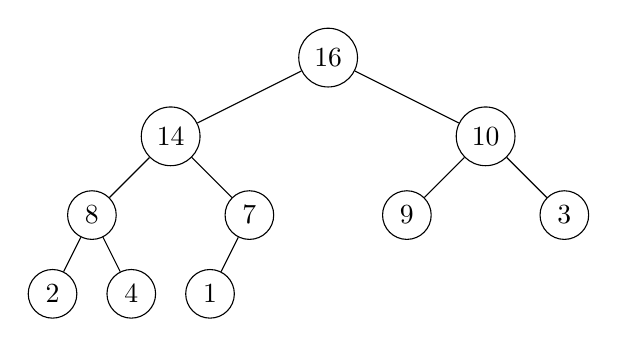
\begin{tikzpicture}
	[
	scale=1.0,
	align=center,
	every node/.style={circle, fill=white, draw=black}
	]
		% level 1
		\node (n1) at 	(3.5, -1) {16};
		
		% level 2
		\node (n2) at 	(1.5, -2) {14};
		\node (n3) at 	(5.5, -2) {10};
		
		% level 3
		\node (n4) at 	(0.5, -3) {8};
		\node (n5) at 	(2.5, -3) {7};
		\node (n6) at 	(4.5, -3) {9};
		\node (n7) at 	(6.5, -3) {3};
		
		% level 4
		\node (n8) at 	(0, -4) {2};
		\node (n9) at 	(1, -4) {4};
		\node (n10) at 	(2, -4) {1};
		% \node (n11) at 	(3, -4) {11};
		% \node (n12) at 	(4, -4) {12};
		% \node (n13) at 	(5, -4) {13};
		% \node (n14) at 	(6, -4) {14};
		% \node (n15) at 	(7, -4) {15};
		
		% drawing code
		\foreach \from/\to in {n1/n2,n1/n3} \draw (\from) -- (\to);
		\foreach \from/\to in {n2/n4,n2/n5,n3/n6,n3/n7} \draw (\from) -- (\to);
		\foreach \from/\to in {n4/n8,n4/n9,n5/n10} \draw (\from) -- (\to);
	\end{tikzpicture}
	\caption{Example of a (binary-)heap visualized as a tree}
	\label{fig:heap-tree}
\end{figure}
...

\section{Priority Queues}
A priority queue is an abstract data structure, which sorts and maintains a
set of data in such a way, that the data is prioritized. It is an important
distinction to make that a priority queue isn't a particular data structure,
but rather a class of data structures. Data structures that work well with
this notion include stacks, heaps, self-organizing lists, etc. We will focus
mainly on heaps.

A heap, however, is not a priority queue in and of itself, it must adhere to
a set of properties, and that is either the max- or min-heap properties.
\begin{description}
	\item \textbf{Max-Heap} The key of a node is greater than or equal to the
keys of its children.
	\item \textbf{Min-Heap} The key of a node is less than or equal to the
keys of its children.
\end{description}
As the max- and min heaps are defined by the procedures performed on them, we
must show that the their property is maintained by each of these procedures.

% pseudo-code for building and maintaining a max- or min-heap (*-heapify and
% build-*-heap, along with explanation for these.

\section{Procedures}
These are the procedures that are supported by max- or min-heaps.

\subsection{Insertion}
...

% TODO: pseudo-code, complexity

\subsection{Extraction}
When we want to extract an element out of a heap, because of its practical use
we are typically interested only in the root node. Getting the root node is a
trivial problem, we simply return the element at index zero - for a max-heap,
this would be the element with the largest key in the set, vice versa for a
min-heap.

% TODO: pseudo-code, complexity

\subsection{Increase key}
...

% TODO: pseudo-code, complexity

% TODO: prove that all procedures maintain the max- or min-heap property

